% Compile with: pdflatex report.tex
\documentclass[12pt,a4paper]{article}
\usepackage[margin=1in]{geometry}
\usepackage{listings}
\usepackage{xcolor}
\usepackage{graphicx}
\usepackage{amsmath}
\usepackage{tabularx}
\usepackage{longtable}
\usepackage[hidelinks]{hyperref}
\usepackage{tikz}
\usepackage{float}
\usepackage{inputenc}
\usetikzlibrary{arrows.meta,automata,positioning}

% Preamble

% --- CORRECT and VERIFIED Custom style for Lex/Flex (.l) files ---

\definecolor{codegreen}{rgb}{0,0.6,0}
\definecolor{codegray}{rgb}{0.5,0.5,0.5}
\definecolor{codepurple}{rgb}{0.58,0,0.82}
\definecolor{backcolour}{rgb}{0.95,0.95,0.92}


\lstdefinestyle{flex}{
    backgroundcolor=\color{backcolour},   
    commentstyle=\color{codegreen},
    keywordstyle=\color{blue},
    numberstyle=\tiny\color{codegray},
    stringstyle=\color{red},
    basicstyle=\ttfamily\small,
    breaklines=true,                 
    numbers=left,                    
    frame=single,
    language=C
}


\title{\textbf{A Report on\\Compiler Design Lab (CS304): Mini Project\\Phase 1}}
\author{
Abhiram Suresh (Roll No: 231CS202)\\
Advaith Nair (Roll No: 231CS205)\\
Arjun Rijesh (Roll No: 231CS212)\\[0.5cm]

\includegraphics[width=6cm]{nitk_logo.png} \\[0.5cm]
\textbf{Department of Computer Science and Engineering}\\
\textbf{National Institute of Technology Karnataka}\\
Surathkal, Mangaluru - 575025\\[0.5cm]
\textbf{15-August-2025}\\[5cm]
}
\date{}

\lstset{
  basicstyle=\ttfamily\small,
  breaklines=true,
  tabsize=2,
  frame=single,
  showstringspaces=false
}

\begin{document}
\maketitle

\vspace{5cm}

\section{Introduction}
This report presents the implementation of a lexical analyzer for the C programming
language using Flex. A lexical analyzer forms the first phase of a compiler,
where the source program is read as a stream of characters and transformed into a
sequence of tokens.

\subsection{Lexical Analysis}
Lexical analysis is the process of converting a sequence of raw characters into a sequence of structured tokens. A lexical analyzer performs this transformation
by scanning the input character by character, grouping them into meaningful units
(tokens), and categorizing them according to their role in the programming language.\\
The lexical analysis phase is crucial because it provides the foundation for the subsequent compilation stages, including syntax analysis, semantic analysis, and code generation. By filtering out irrelevant details (such as whitespace and comments), building symbol and constant tables, and detecting invalid inputs early, the lexical analyzer ensures that later phases, like semantic analysis, receive a stream of tokens accompanied by valuable contextual metadata.\\
Our implementation not only performs token recognition, but also integrates the construction of a \textbf{symbol table} to record identifiers and their frequencies of use, as well as a \textbf{constant table} to store details about constants, including their type, value, and line number of occurrence. In addition, it provides mechanisms for handling nested comments, reporting lexical errors such as invalid tokens and unterminated comments, and maintaining accurate line numbers for error reporting.

\subsection{Tokens \& Lexemes}
\textbf{Token:} A pair consisting of a token name and an optional attribute value that uniquely identifies a sequence of characters.\\
\\
\textbf{Lexeme:} The actual sequence of characters in the source program that matches the pattern for a token.\\
\\
In our mini-project, we have implemented a lexical analyzer for the C language using \textbf{Flex}. The scanner can recognize the following:
\begin{itemize}
    \item Identifiers - Variable names, function names, and other user-defined names;
    these are stored in the symbol table along with their frequency of occurrence
    \item Preprocessor Directives - Lines beginning with the \# symbol, such as \#include
    and \#define
    \item Keywords - Reserved words in C (e.g., int, float, if, while, etc.)
    \item Constants - Numeric constants (integer, floating-point, hexadecimal, octal),
    character constants, and string literals; these are recorded in the constant table
    with their type, value, and line number
    \item Operators - Arithmetic, relational, logical, bitwise, assignment, increment/decre-
    ment, pointer, address-of, and member operators
    \item Punctuation - Parentheses, braces, brackets, semicolons, and commas
    \item Comments - single-line and multi-line including nested multi-line comments
\end{itemize}
For example, in:
\begin{lstlisting}[language=C]
int x = 10;
\end{lstlisting}
``int'' is a keyword token, ``x'' is an identifier token, and ``10'' is a constant token. \vspace{0.5cm}

\section{Code Listing}

\lstinputlisting{src/Scanner/scanner.l}

\vspace{2cm}


\section{DFA Diagram}

\begin{figure}[H]
    \centering % This command centers the image
    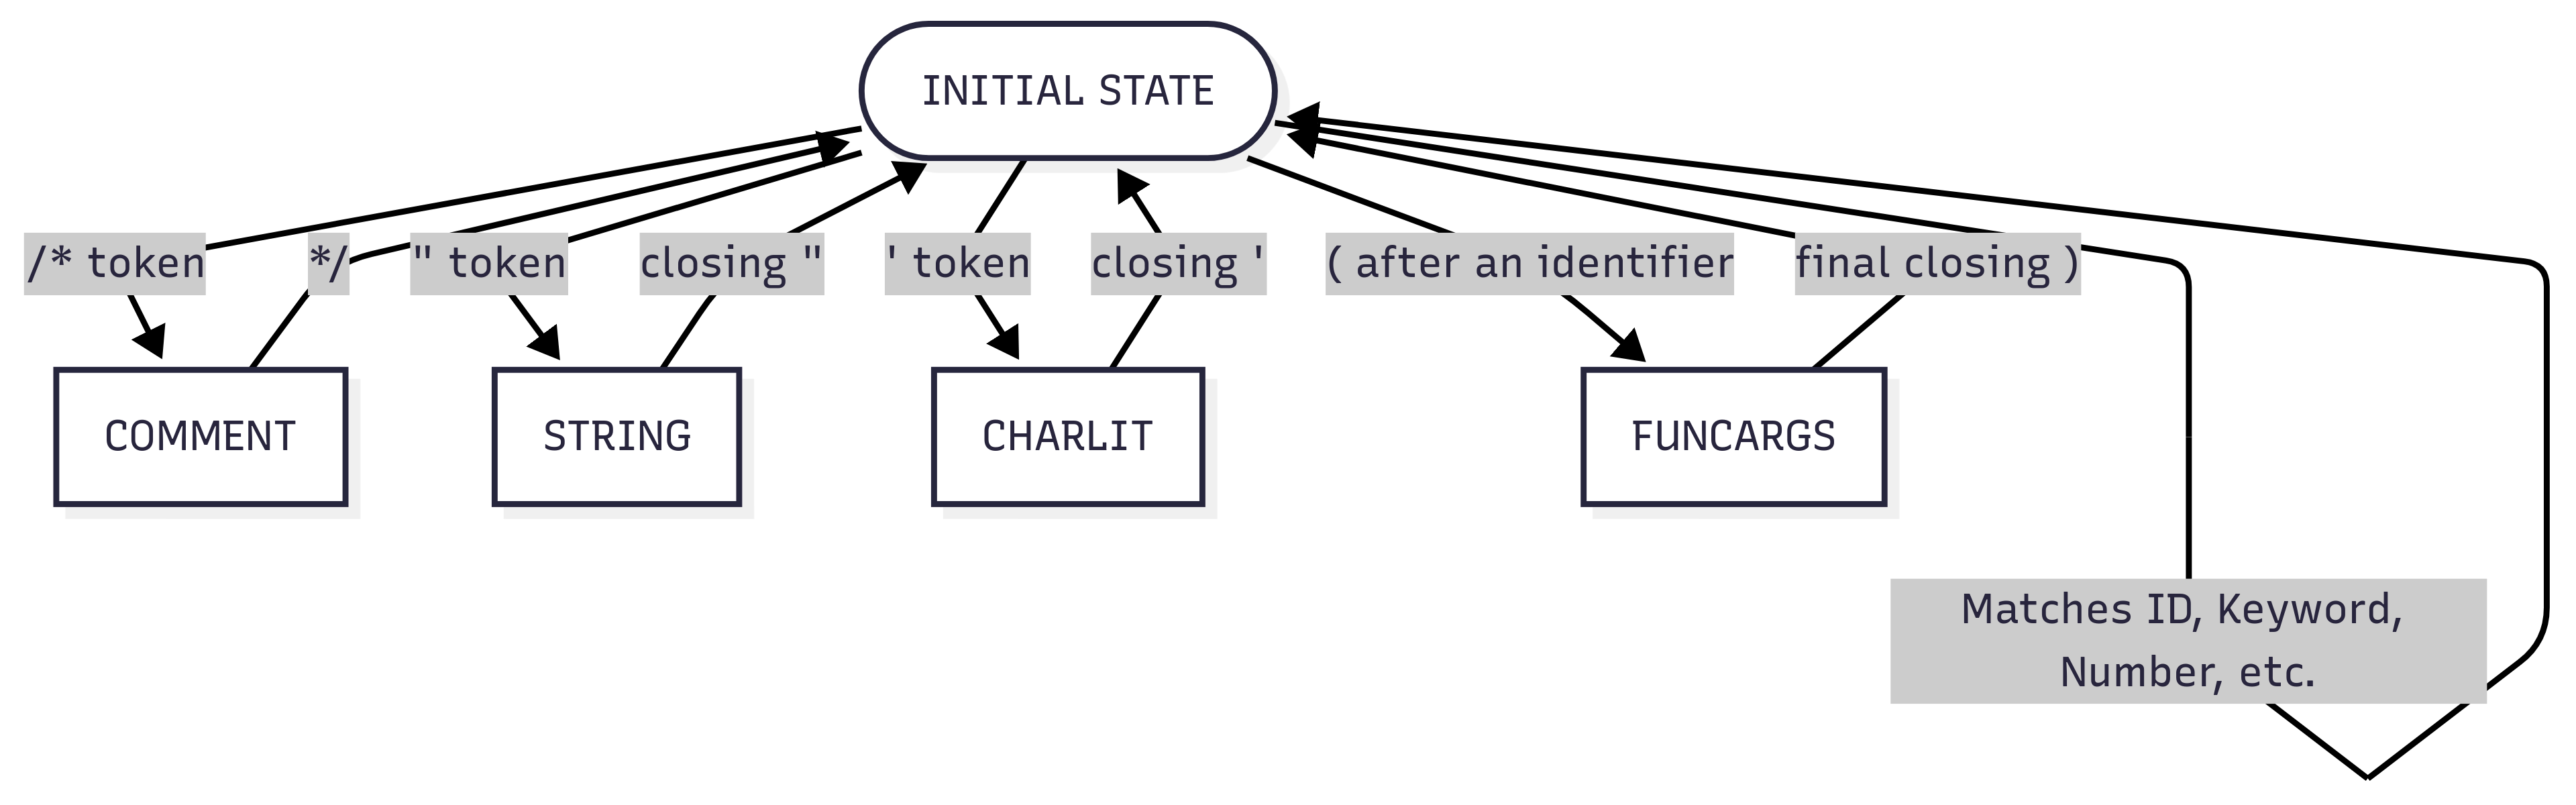
\includegraphics[width=1\textwidth]{Initial States.png}
    \caption{FULL DFA}
\end{figure}

\begin{figure}[H]
    \centering % This command centers the image
    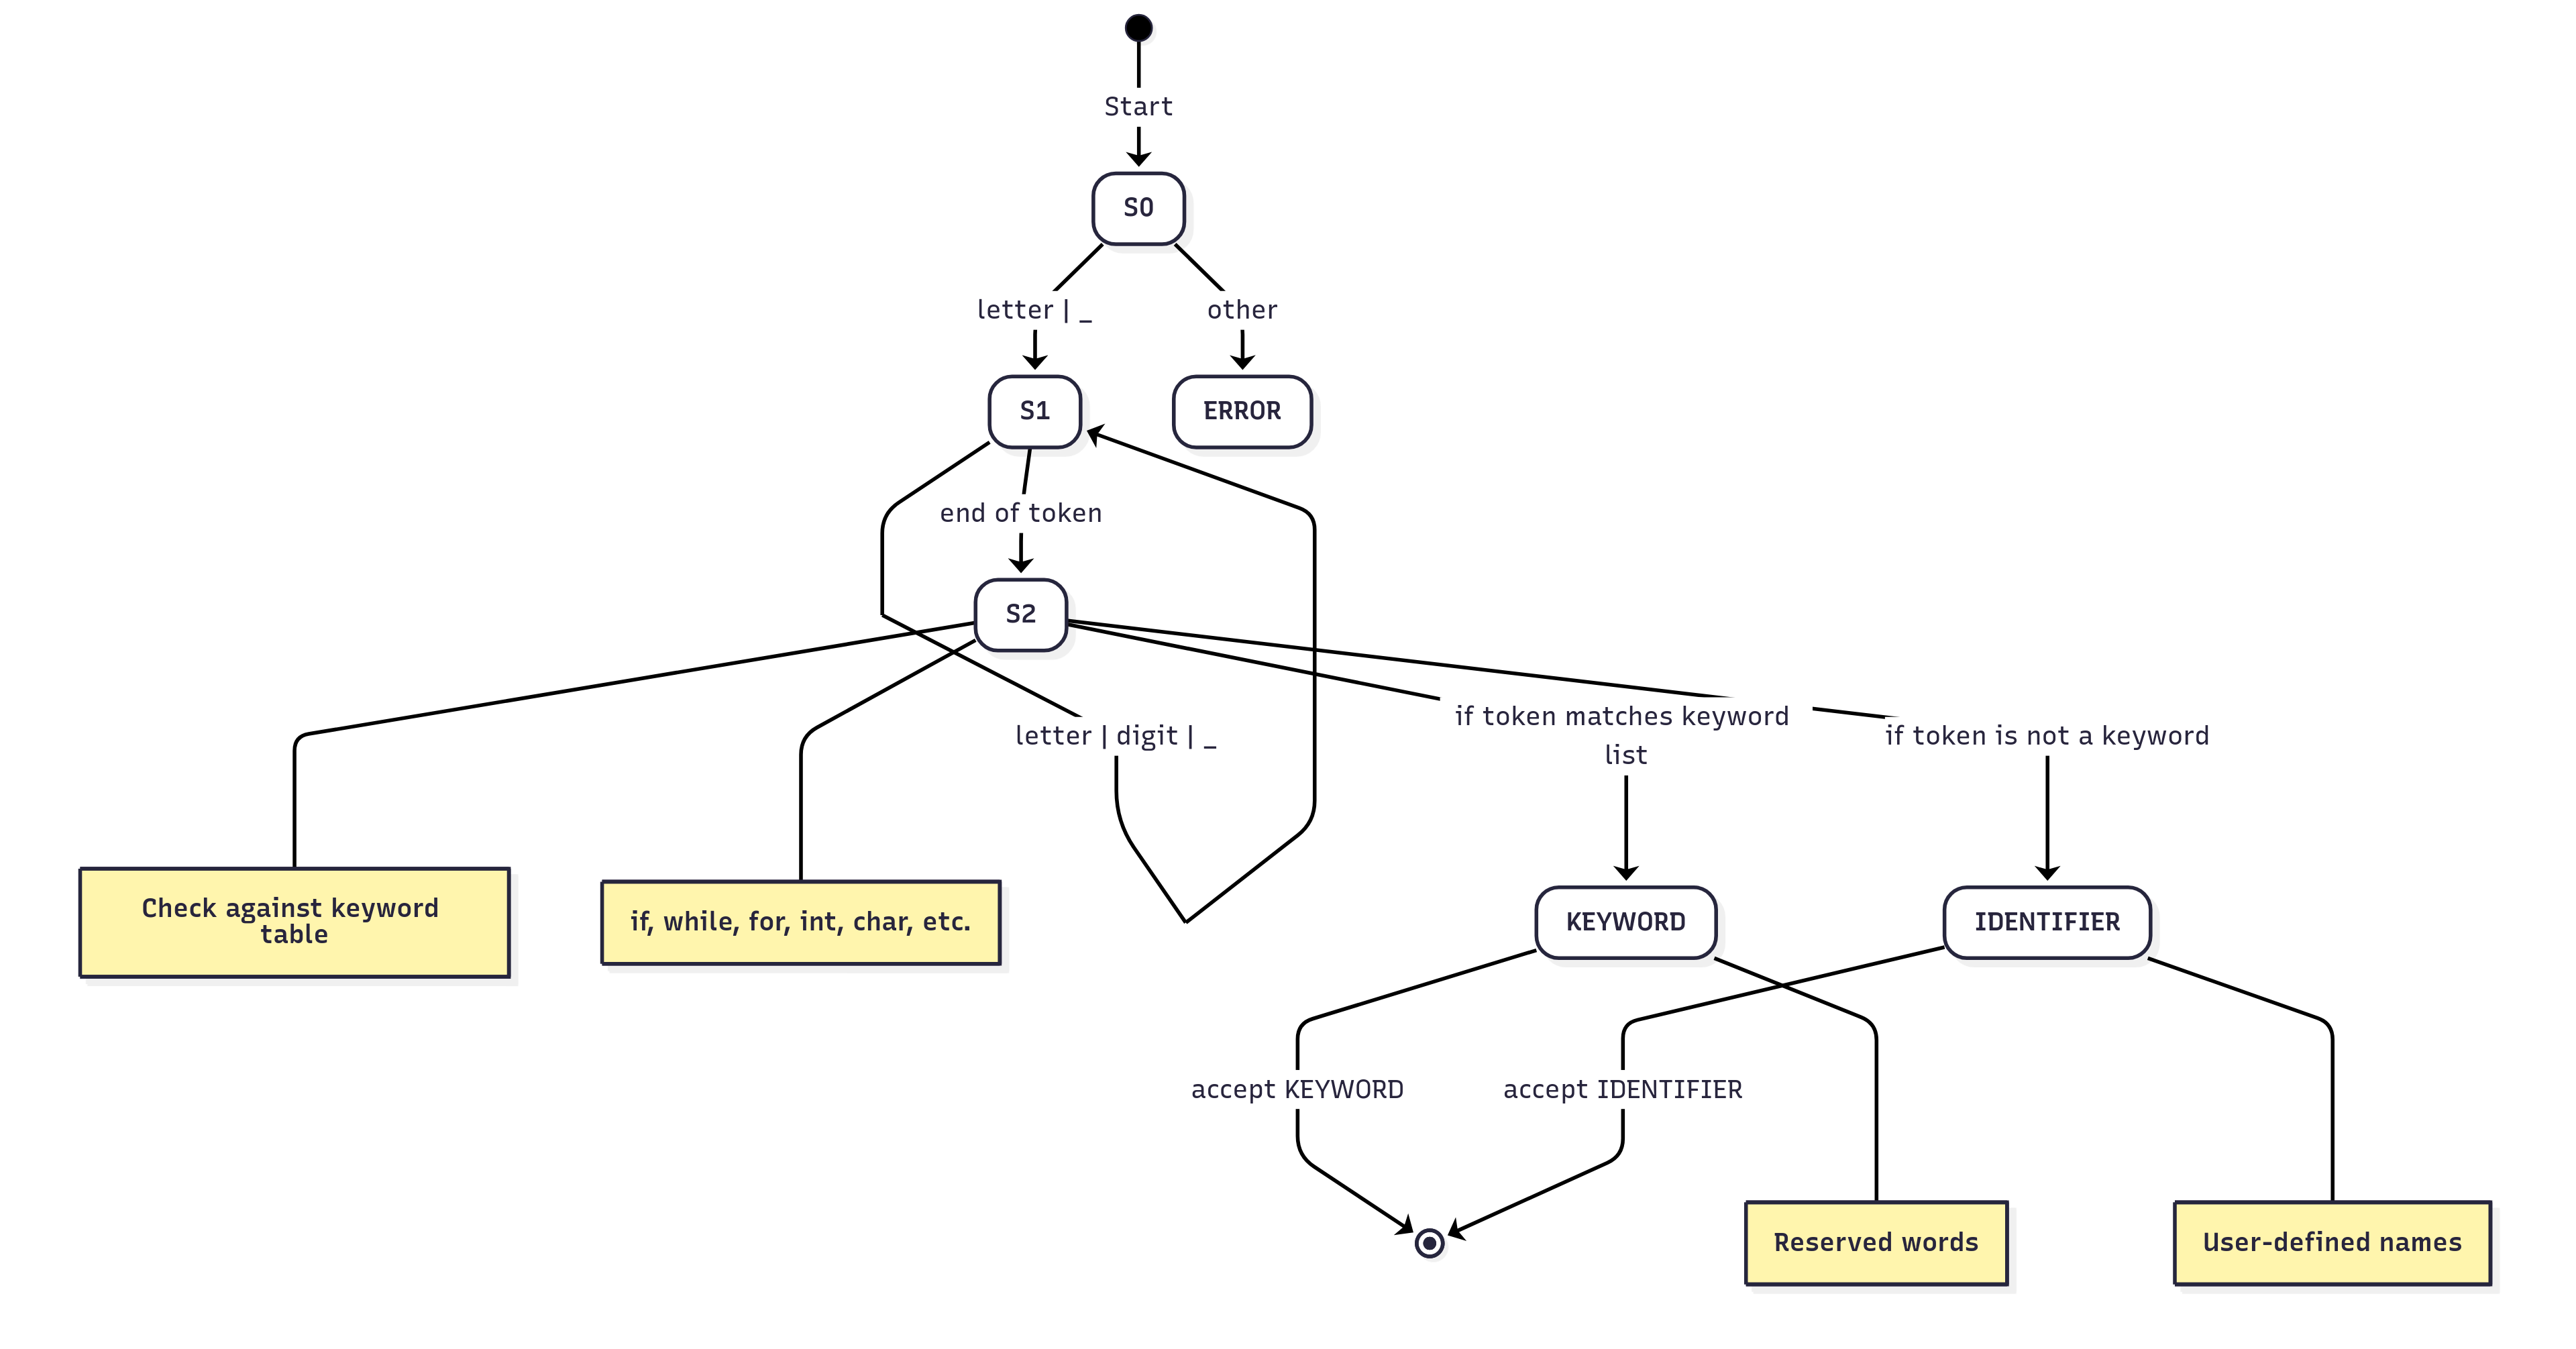
\includegraphics[width=1\textwidth]{IDKEY.png}
    \caption{Identifier vs Keywords}
\end{figure}




The behavior of the DFA upon entering the \texttt{INITIAL STATE} can be summarized as follows:

\begin{itemize}
    \item \textbf{Start of Tokenization:} Every time the analyzer looks for a new token, it begins in this state.

    \item \textbf{Specific Delimiters:} The initial character(s) route the DFA to a dedicated state for handling complex tokens:
    \begin{itemize}
        \item If the input starts with `/*`, the DFA transitions to the \texttt{COMMENT} state to process a multi-line comment.
        \item A `"` (double quote) transitions to the \texttt{STRING} state to handle string literals.
        \item A `'` (single quote) transitions to the \texttt{CHARLIT} state for character literals.
    \end{itemize}

    \item \textbf{Context-Sensitive Tokens:} In some cases, the transition depends on context. For example, an opening parenthesis `(` after an identifier transitions the DFA to the \texttt{FUNCARGS} state to parse function arguments.

    \item \textbf{General Tokens:} For most other inputs, such as letters or digits that begin an identifier, keyword, or number, the DFA follows a general path to recognize these common tokens.

    \item \textbf{Return to Initial State:} After a token is fully recognized (e.g., upon reaching a closing `*/` for a comment or the final `"` for a string), the lexeme is processed, and the DFA returns to the \texttt{INITIAL STATE} to begin scanning for the next token. This is represented by the "closing" arrows returning to the top.
\end{itemize}

\vspace{0.5cm}

\section{Assumptions}
\addcontentsline{toc}{section}{6 Assumptions}

The following assumptions were made in addition to the C language specification:
\begin{enumerate}
    \item Identifiers begin with a letter or underscore, followed by letters, digits, or underscores.
    \item Numbers are recognized in decimal, octal (leading 0), and hexadecimal (prefix 0x) formats.
    \item Floating point numbers must include a decimal point.
    \item Strings are enclosed in double quotes and cannot span multiple lines.
    \item Nested comments are supported.
    \item Preprocessor directives are assumed to appear at the start of a line.
    \item Cant differentiate between the deference operator and arithmetic operator *
\end{enumerate}

\section{Handling of Strings, Comments, and Errors}

\subsection{String and Character Literal Handling}
The scanner utilizes exclusive start conditions to parse string and character literals, ensuring that special characters are not misinterpreted.
\begin{itemize}
    \item \textbf{State Transition:} An opening double-quote (\texttt{"}) transitions the scanner into the \texttt{STRING} state. Similarly, an opening single-quote (\texttt{'}) enters the \texttt{CHARLIT} state. The \texttt{yyless(0)} function is used to ensure the quote itself is included in the token text.
    \item \textbf{Tokenization:} Once in the respective state, a pattern matches the entire literal content until the closing quote. The matched literal is then printed as a token and added to the constant table.
    \item \textbf{Error Handling:} If a newline character is encountered before the literal is terminated by its closing quote, it is considered an error. An "Unterminated string literal" or "Unterminated char literal" message is printed to standard error, and the scanner returns to the \texttt{INITIAL} state.
\end{itemize}

\subsection{Comment Handling}
The scanner is capable of processing both single-line and multi-line C-style comments.
\begin{itemize}
    \item \textbf{Single-Line Comments:} Any text beginning with \texttt{//} until the end of the line is matched and ignored.
    \item \textbf{Multi-Line Comments:} An opening \texttt{/*} transitions the scanner into the \texttt{COMMENT} start condition.
    \item \textbf{Nested Comment Support:} The scanner correctly handles nested multi-line comments. It initializes a \texttt{depth} counter to 1 and increments it for each subsequent \texttt{/*} and decrements it for each \texttt{*/}. The scanner only returns to the \texttt{INITIAL} state when the depth counter reaches zero.
    \item \textbf{Error Handling:} If the end of the file is reached while the scanner is still in the \texttt{COMMENT} state (i.e., the depth is non-zero), an "Unterminated comment" error is reported.
\end{itemize}

\subsection{General Error Handling}
In addition to specific cases for literals and comments, the scanner has general mechanisms for error reporting.
\begin{itemize}
    \item \textbf{Invalid Tokens:} A catch-all rule, \texttt{.}, matches any single character that does not conform to any of the other defined rules. This triggers an "Invalid token" error message, which includes the offending character(s).
    \item \textbf{File Handling Errors:} In the \texttt{main} function, if a source file is provided as a command-line argument but cannot be opened, the \texttt{fopen} call will fail. This condition is checked, and the system error is reported via \texttt{perror} before the program exits with a status of 1.
\end{itemize}
\vspace{5cm}

\section{Results}

\subsection*{Test Case 1}
\textbf{Input:}
\begin{lstlisting}[style=flex]
#include <stdio.h>
unsigned long fact(int n);
int add(int x, int y) { return x + y; }
int arr[10][20];
int main()
{
    int r = add(3, 5);
    printf("%d\n", r);
    return 0;
}
unsigned long fact(int n)
{
    if (n <= 1)
        return 1;
    return n * fact(n - 1);
}
\end{lstlisting}

\begin{figure}[H]
    \centering
    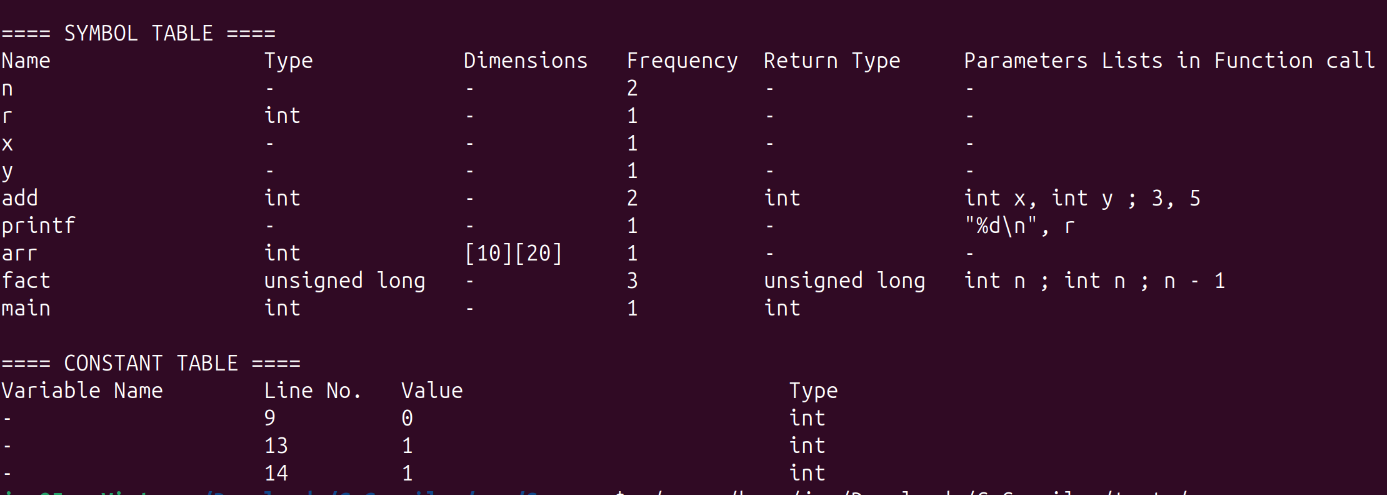
\includegraphics[width=0.9\linewidth]{functions.png}
\end{figure}

\subsection*{Test Case 2}
\textbf{Input:}
\begin{lstlisting}[style=flex]
#include <stdio.h>
int main()
{
    int a = 09;    // octal invalid in C (but lexer will just see a number token)
    char c = 'ab'; // invalid char literal (lexer will catch as char literal or error depending on quotes)
    $invalid = 5;  // invalid token starting with $
    "unterminated string
    /* unterminated comment
    return 0;
}
\end{lstlisting}

\textbf{Output:}
\begin{figure}[H]
    \centering
    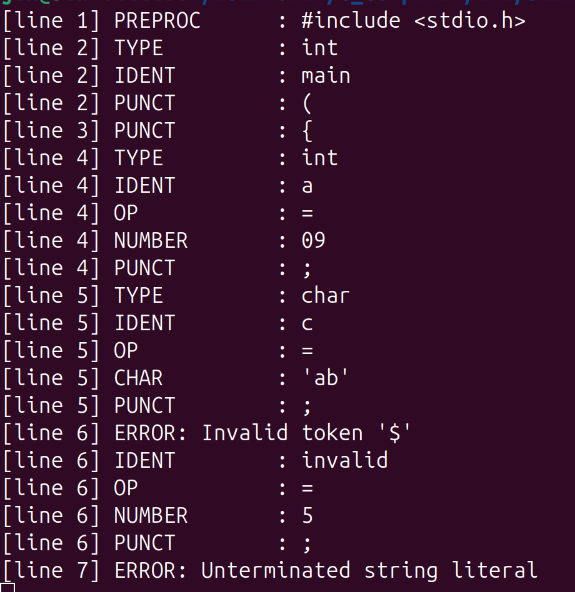
\includegraphics[width=0.9\linewidth]{errors.png}
\end{figure}
\vspace{0.5cm}

\section{Conclusion}
In this phase of the mini project, we successfully implemented a lexical analyzer using Flex. The analyzer correctly identifies tokens, generates symbol and constant
tables, and reports lexical errors with line numbers. The test cases demonstrate the
correctness of token recognition and the robustness of error handling.
Future work will focus on integrating this lexical analyzer with parsing and se-
mantic analysis modules, eventually leading to a complete compiler front-end imple-
mentation.

\end{document}